% !TeX encoding = UTF-8
% !TeX spellcheck = en_US
% !TeX root = presentation.tex

\subsection{Simulation}

\begin{frame}{Simulation}
    \begin{itemize}
        \item Simple Two Dimensional Robot (STDR) simulator	
        \item Tasks  performed:
        \begin{itemize}
            \item Map Building
            \item Localization
        \end{itemize}
    \end{itemize}
    
    \centering
    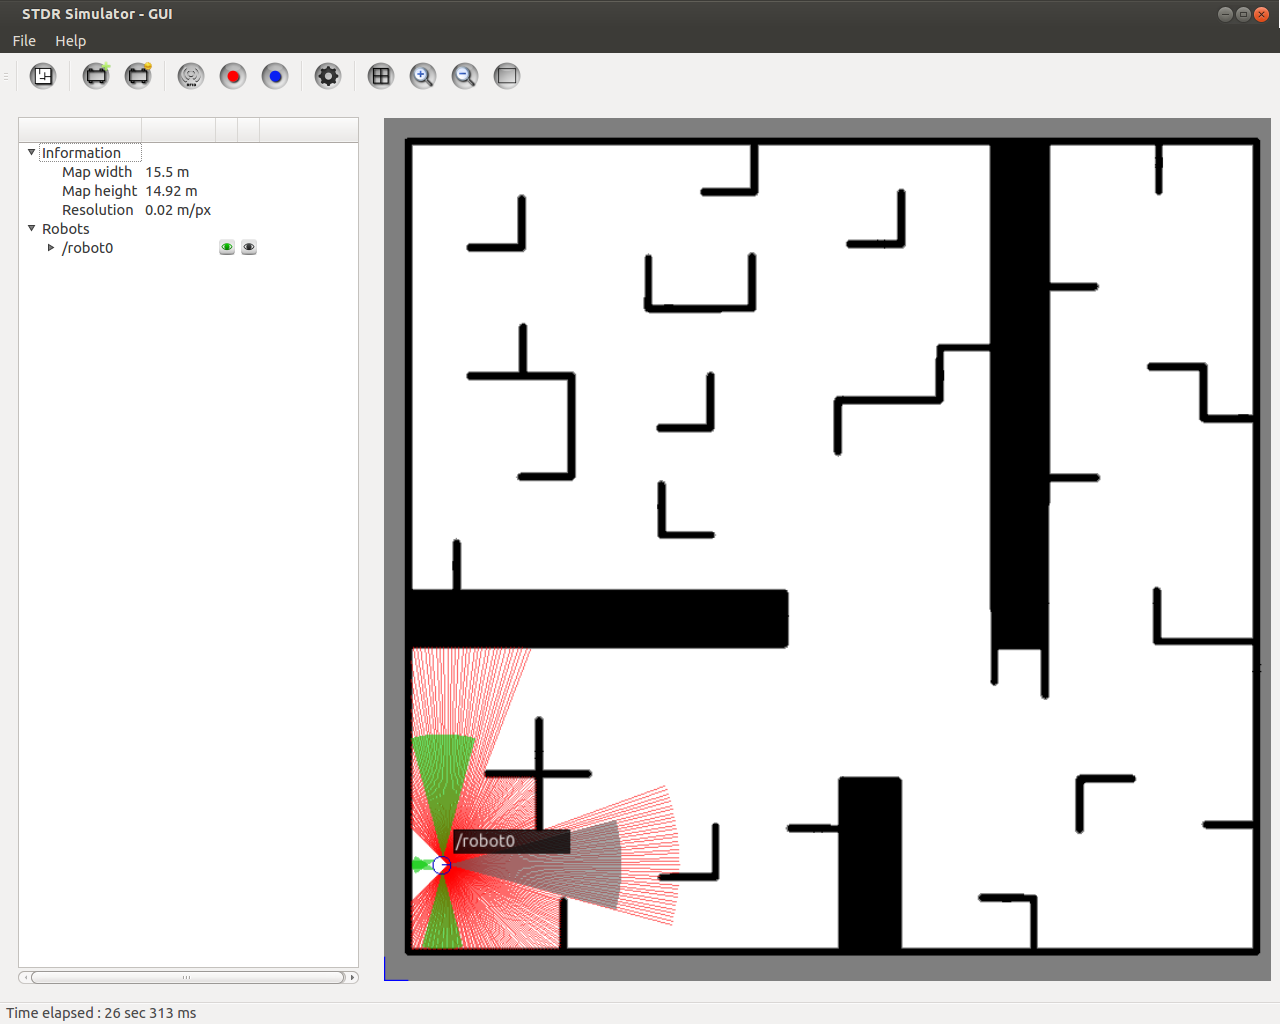
\includegraphics[width=90mm,height=55mm]{gfx/stdr_simulator}
    
\end{frame}
%---------------------------------------------------------------
\begin{frame}{Map building I}
    \begin{itemize}
        \item Gmapping is used to build 2D occupancy grid map 
        \item RAO-BLACKWELLIZED Mapping 
        \begin{itemize}
            \item Individual map is associated to every sample
            \item Each map is built given the observations and the
trajectory
            \item ????

        \end{itemize}
        \item Map Server
        \begin{itemize}
            \item Provides map saver utility, to save generated map in files(yaml and pgm)
            \item Offers map data as a ROS Service
        \end{itemize}
        
    \end{itemize}
\end{frame}
%----------------------------------------------------------------
\begin{frame}{Localization I}
    \begin{itemize}
        \item Adaptive Monto Carlo Localization(AMCL) is used to localize the robot
        \item Uses particle filter to track the pose of robot
        \begin{itemize}
          \item Distribute samples according to initial pose
          \item For each particle, predict next pose from motion model and add random noise
          \item Update each particle\'s weight based on 
likelihood of getting the sensor readings from
that particle\'s hypothesis
          \item Resample new set of particles according to its weight	
        \end{itemize}
        \item What it needs?
        \begin{itemize}
            \item Laser scans
            \item Initial pose
            \item Transforms
            \item Map 
        \end{itemize}
    \end{itemize}
\end{frame}
%----------------------------------------------------------------
\begin{frame}{Localization I}
\begin{itemize}
	\item \textbf{Problems}
	\begin{itemize}
		\item Amcl could not find laser data on /scan topic
		\item Amcl node crushes after some time
		\item Amcl is not working
	\end{itemize}
	\item \textbf{Solutions}
	\begin{itemize}
		\item Remap /scan\_front and /scan\_rear to /scan topic
		\item Because of incorrect transformations provided by stdr simulator
		\item Parameter odom\_model\_type should be omni\-corrected
	\end{itemize}
\end{itemize}
\end{frame}